\chapter{Model, Algorithms, and
Methodology}

Chapter 2 placed the problem in its field. This chapter fixes the
precise model and notation used throughout (§3.1), details the
algorithms as we implement them (§3.2), the prediction objects and
structured error models (§3.3), the consistency/robustness measures
(§3.4), and the experimental harness (§3.5). It closes by validating the
harness against the published Borodin et al.~figures before any
contribution is built on it (§3.6).

\section{The known-i.i.d. model,
precisely}

There is a set \(R\) of \(n\) offline \textbf{resources} and a
\textbf{type graph} on \(r\) online \textbf{types}; type \(\ell\) has
neighborhood \(N(\ell)\subseteq R\). An instance is generated by drawing
\(m\) arrivals i.i.d. from a distribution \(p\) over the \(r\) types;
the \(i\)-th arrival reveals its type (hence \(N(\cdot)\)) and must be
matched to a currently unmatched resource in its neighborhood,
immediately and irrevocably, or left unmatched. The type graph and \(p\)
are known to the algorithm; the realized arrival sequence is not.
Following the standard \emph{integral-types} convention, the default is
\(m=n\) with uniform \(p\), so each type's expected count is an integer;
the classical setting has \(r=n\) (each offline vertex a distinct type),
and the \emph{few-types} setting used for the histogram-advice
experiments has \(r\ll n\).

The performance measure is the \textbf{competitive ratio}, computed per
instance and then averaged:
\(\rho(\mathrm{ALG}) = \mathbb E\bigl[|\mathrm{ALG}|/|\mathrm{OPT}|\bigr]\),
where \(\mathrm{OPT}\) is a maximum matching of the realized instance,
computed exactly by Hopcroft--Karp \autocite{hopcroftkarp1973}.
Averaging per-instance ratios is the natural convention under paired
trials (§3.5), since on a given instance every algorithm is divided by
the same exactly-computed optimum. It differs in principle from the
ratio of expectations
\(\mathbb E[|\mathrm{ALG}|]/\mathbb E[|\mathrm{OPT}|]\) that an
experimental study might report instead, so we measured the gap: across
nine algorithm-by-quality cells spanning both prediction families, the
two conventions agree to within \(6\times10^{-5}\), two orders of
magnitude below the confidence intervals we report, so no number in this
thesis depends on the choice (\texttt{scripts/run\_metric\_check.py},
§A.2). The advice-free baseline throughout is KVV Ranking, whose ratio
we write \(\rho_{\mathrm{base}}\) (the \textbf{baseline strength}).

The notation recurs throughout the thesis and is collected here for
reference:

{ % do not increment counter
\begin{longtable}[]{@{}
  >{\raggedright\arraybackslash}p{(\linewidth - 4\tabcolsep) * \real{0.3333}}
  >{\raggedright\arraybackslash}p{(\linewidth - 4\tabcolsep) * \real{0.3333}}
  >{\raggedright\arraybackslash}p{(\linewidth - 4\tabcolsep) * \real{0.3333}}@{}}
\toprule\noalign{}
\begin{minipage}[b]{\linewidth}\raggedright
symbol
\end{minipage} & \begin{minipage}[b]{\linewidth}\raggedright
meaning
\end{minipage} & \begin{minipage}[b]{\linewidth}\raggedright
typical value
\end{minipage} \\
\midrule\noalign{}
\endhead
\bottomrule\noalign{}
\endlastfoot
\(n\) & offline resources & 1000--2000 \\
\(r\) & online request types & \(r=n\) (classical), \(r=8\)
(few-types) \\
\(m\) & arrivals in one instance & \(m=n\) \\
\(p\) & known distribution over types & uniform unless stated \\
\(\mu\) & predicted resource degrees (degree prediction) & --- \\
\(\hat c\) & predicted type counts (histogram prediction) & --- \\
\(k\) & length of the prefix a test may inspect & \(k=200\) \\
\(\eta\) & strength of the injected prediction error &
\(\eta\in[0,1]\) \\
\(\rho_{\mathrm{base}}\) & Ranking's ratio on that instance family (the
floor) & 0.89--0.99 \\
\end{longtable}
}

\section{Algorithms}

All greedy-type algorithms are instances of one primitive: given a total
order (\textbf{rank}) on the resources, GreedyWithPermutation matches
each arrival to its available neighbor of minimum rank. This makes the
algorithm family a single code path parameterized by the rank, which is
important both for a fair comparison and for the theory.

\begin{itemize}
\item
  \textbf{Advice-free baselines.} SimpleGreedy (identity rank), Ranking
  (uniformly random rank; the baseline), and the stochastic-matching
  algorithms Feldman and Jaillet--Lu, which precompute a suggested
  matching by max-flow: Feldman from a cap-\(\{2,1,2\}\) network, whose
  unit-flow subgraph splits into a blue and a red matching; Jaillet--Lu
  from a cap-\(\{3,2,3\}\) network, whose fractional solution gives a
  per-type list of resources to try in order. Each of the two has a
  \emph{non-greedy} variant (follow the suggestion only) and a
  \emph{greedy} variant (fall back to any available neighbor).
\item
  \textbf{Degree predictions.} MinPredictedDegree (MPD) is
  GreedyWithPermutation ranked by ascending predicted degree
  \(\mu\in\mathbb R^R\). Constant \(\mu\) gives Ranking; the true
  realized degrees give the consistency ceiling (MinDegree). The
  \textbf{augmentations} Feldman(MPD) and JailletLu(MPD) use the MPD
  rank only as the tie-break of the greedy fallback.
\item
  \textbf{Type-histogram advice and test-and-fallback.} From a count
  vector \(\hat c\) over types we build an advice matching \(\hat M\)
  and record its per-type partners. FollowPrediction routes every
  arrival to its type's predicted partner; TestAndMatch (Choo and BEM)
  does the same over a length-\(k\) prefix, tests the empirical
  \(\ell_1\) distance between the prefix frequencies and
  \(q=\hat c/\lVert\hat c\rVert_1\) against a threshold \(\tau\), then
  continues or falls back to Ranking. The Chłędowski-style dynamic
  combiner is ported as a benchmarked baseline, not a contribution.
\end{itemize}

This last point is the mechanism behind the structural robustness of
Chapter 4. Because the prediction only decides between otherwise
equivalent choices, the worst-case-optimal base matching carries most of
the load and a bad prediction can affect only the tie-breaks. This
limits the downside, but also caps the upside when the prediction is
good.

\section{Prediction objects and structured error
models}

The families consume different prediction objects (degree vectors
\(\mu\) and type histograms \(\hat c\)), so each is corrupted by its own
knob and reported in a parallel panel. For \(\mu\) we use four
structured error models, each driven by a strength \(\eta\in[0,1]\) and
each returning both an \(\ell_1\) \emph{magnitude} error and a
normalized \textbf{Kendall-\(\tau\) order error}:

{ % do not increment counter
\begin{longtable}[]{@{}
  >{\raggedright\arraybackslash}p{(\linewidth - 4\tabcolsep) * \real{0.3333}}
  >{\raggedright\arraybackslash}p{(\linewidth - 4\tabcolsep) * \real{0.3333}}
  >{\raggedright\arraybackslash}p{(\linewidth - 4\tabcolsep) * \real{0.3333}}@{}}
\toprule\noalign{}
\begin{minipage}[b]{\linewidth}\raggedright
model
\end{minipage} & \begin{minipage}[b]{\linewidth}\raggedright
construction at strength \(\eta\)
\end{minipage} & \begin{minipage}[b]{\linewidth}\raggedright
effect on the induced order
\end{minipage} \\
\midrule\noalign{}
\endhead
\bottomrule\noalign{}
\endlastfoot
random-flip & independently, with probability \(\eta\), replace an entry
of \(\mu\) by a uniform draw from \([\min\mu,\max\mu]\) & grows with
\(\eta\); \(\eta=1\) is a constant-quality predictor, i.e.~Ranking \\
systematic-bias & monotone rescale \(\mu\leftarrow\mu\cdot(1+\eta)\) &
none: Kendall-\(\tau\equiv0\) by construction, while the \(\ell_1\)
magnitude grows linearly \\
adversarial & for an \(\eta\)-fraction of resources \(u\in R\), reflect
\(\mu(u)\leftarrow(\min\mu+\max\mu)-\mu(u)\) & the most order-damaging
perturbation at a given fraction; \(\eta=1\) reverses the order \\
distribution-drift & blend toward the degrees of an independently drawn
graph of the same family,
\(\mu\leftarrow(1-\eta)\mu+\eta\mu_{\mathrm{alt}}\) & grows with
\(\eta\), but in a correlated way rather than entry-by-entry \\
\end{longtable}
}

For \(\hat c\) we blend the realized counts toward a concentrated random
target by a fraction \(\eta\in[0,1]\), reporting the induced
\(\ell_1(p,q)\). Because MPD depends on \(\mu\) only through the induced
order, the order/magnitude distinction is the axis of Chapter 5.

\section{Consistency and robustness}

For a prediction-consuming algorithm, \textbf{consistency} is its ratio
under perfect advice and \textbf{robustness} is its worst-case ratio
under adversarial advice. Operationally we cannot sweep every
adversarial prediction, so in the experiments robustness is reported as
the minimum over our corruption levels, an upper bound on the true worst
case and therefore a generous reading of an algorithm's safety. A useful
algorithm is consistent and never (much) below \(\rho_{\mathrm{base}}\);
the tension between the two is the subject of Chapter 6 and of the
outlook in §10.2.

\section{The experimental harness}

The harness is a small, dependency-light Python codebase (NumPy, SciPy,
NetworkX). Every source of randomness draws from its own independent,
reproducible stream, so that within a comparison the only thing that
varies is the prediction and adding an algorithm never disturbs existing
results (Appendix A.1 lists the streams). We use \textbf{paired trials}:
within a comparison, every algorithm and error level reuses the same
graph, arrival sequence, \(\mathrm{OPT}\), and tie-break seed, so
differences are attributable to the prediction alone. Reported ratios
are means over trials with 95\% normal-approximation confidence
intervals, computed per algorithm and error level. Those per-algorithm
intervals are the conservative choice: they under-use the pairing, since
a comparison between two algorithms is really a \emph{paired
difference}, whose interval is narrower whenever the two respond to the
same instances in the same direction. Every comparison the thesis draws
survives under the wider convention (the narrowest margin being
Feldman(MPD)'s \(+0.0044\) against a \(\pm0.0023\) per-algorithm
interval), so nothing in the thesis turns on which is used; §A.2 reports
the measured correlations and paired intervals. Every figure and table
in the thesis is regenerated from a fixed seed by a single script
(Appendix A).

\section{Fidelity check: reproducing Borodin et
al.}

Before building prediction-based algorithms on the harness, we validated
it against the published experimental study of Borodin, Karavasilis and
Pankratov \autocite{borodin2018experimental}. This is a \textbf{fidelity
check, not a contribution}: its purpose is to confirm that the
generators, the i.i.d. sampler, the Hopcroft--Karp optimum, and the
algorithm implementations reproduce the paper's qualitative findings, so
that later differences can be attributed to the algorithms rather than
to infrastructure. Our stack (Python/NetworkX) differs from the paper's
(C++/Edmonds--Karp), so we target \emph{qualitative} agreement,
accepting small absolute differences (\(\le 0.02\)).

We reproduced the core four algorithms (six greedy/non-greedy variants)
on two random graph families at \(n=1000\), \(m=n\), 100 trials per
parameter value (matching the paper's setup), under a single master
seed.

\textbf{Erdős--Rényi (edge probability \(c/n\); the paper's Fig. 9,
partial).} All five of the paper's qualitative claims that we checked
reproduce, with absolute differences below \(0.02\). In detail: sweeping
\(c\) reproduces the characteristic U-shape and its hard case,
SimpleGreedy attains its minimum \(0.864\) at \(c\approx4.9\), and the
greedy variants of the complex algorithms their minima \(\approx0.884\)
at \(c\approx5.3\). Ranking is indistinguishable from SimpleGreedy
(maximum difference \(0.0017\) across all 75 values; the paper omits
Ranking's curve for exactly this reason), and the non-greedy variants
degrade monotonically as \(c\) grows (\(0.986\to0.730\) for Feldman,
\(0.985\to0.760\) for Jaillet--Lu). Every one of the paper's five prose
claims we checked holds (\textbf{Figure 3.1}).

\begin{figure}
\centering
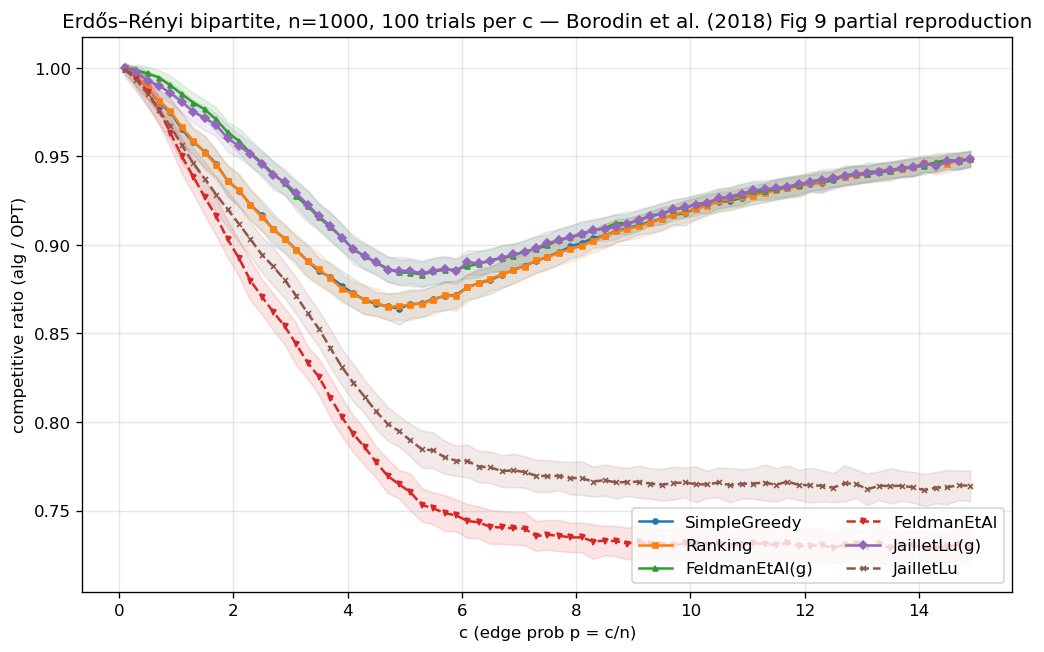
\includegraphics[width=0.65\linewidth,height=\textheight,keepaspectratio,alt={Erdős--Rényi reproduction: the characteristic U-shape, greedy minima near c\textbackslash approx4.9, non-greedy degradation as c grows.}]{../../results/er_full.png}
\caption{Erdős--Rényi reproduction: the characteristic U-shape, greedy
minima near \(c\approx4.9\), non-greedy degradation as \(c\) grows.}
\end{figure}

\textbf{Random left-regular (left-degree \(d\); the paper's Fig. 18,
partial; Figure 3.2).} The pattern repeats with the hard case at \(d=5\)
(SimpleGreedy minimum \(0.890\)), Ranking \(\approx\) SimpleGreedy (max
difference \(0.0013\)), non-greedy degradation as \(d\) grows, and
greedy complex variants \(\approx\) SimpleGreedy asymptotically.

\begin{figure}
\centering
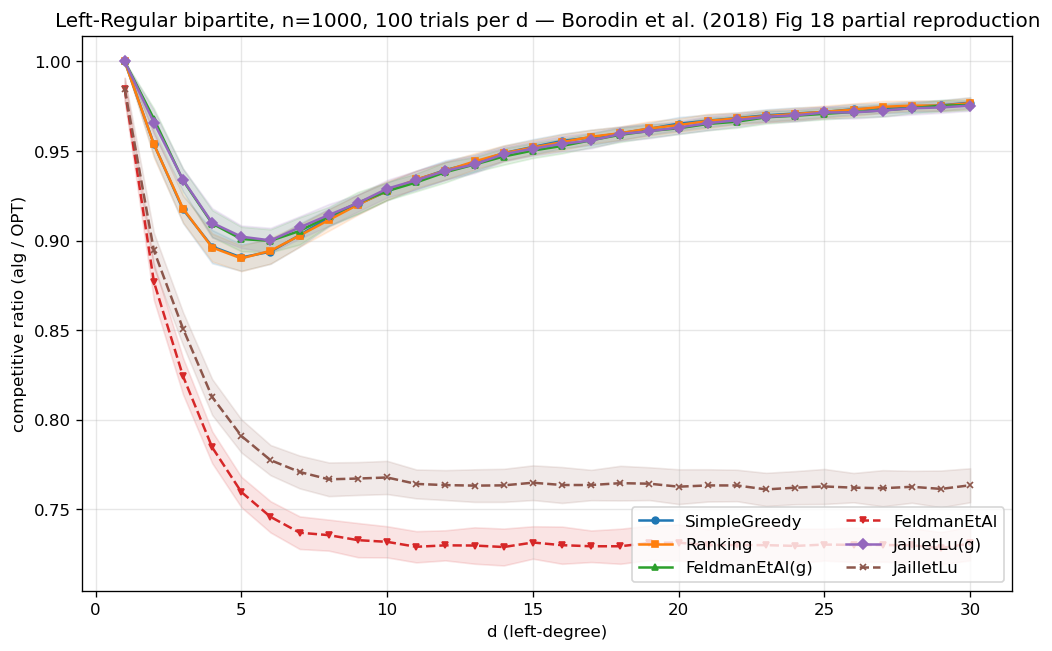
\includegraphics[width=0.65\linewidth,height=\textheight,keepaspectratio,alt={Random left-regular reproduction: the hard case at d=5, Greedy \textbackslash approx Ranking.}]{../../results/left_regular.png}
\caption{Random left-regular reproduction: the hard case at \(d=5\),
Greedy \(\approx\) Ranking.}
\end{figure}

\textbf{A cross-family observation.} Combining the two sweeps surfaces a
non-obvious fact: the non-greedy Feldman and Jaillet--Lu algorithms
converge to the same asymptotic ratio in both families (\(0.730\) and
\(0.760\) respectively, within \(0.001\) across families) and both sit
above their worst-case theoretical bounds (\(0.670\) and \(0.729\)) by
\(+0.06\) and \(+0.03\). The two families happen to converge to the same
value here; we do not investigate whether that is universal. It is, in
any case, an early and concrete instance of the thesis's recurring theme
that the average case is far more benign than the worst case, which the
prediction-error sweeps of later chapters probe in earnest.

\textbf{Verdict.} The harness reproduces the published qualitative
findings on both families, including the locations of the hard cases and
the near-identity of Greedy and Ranking. The foundation is trusted; the
contributions of Chapters 4--9 are built on it. (Full reproduction
tables and the paper-claim checklist are in Appendix A.)
